\documentclass[a4paper, twoside]{report}

%% Language and font encodings
\usepackage[english]{babel}
\usepackage[utf8x]{inputenc}
\usepackage[T1]{fontenc}

%% Sets page size and margins
\usepackage[a4paper,top=3cm,bottom=2cm,left=3cm,right=3cm,marginparwidth=2.0cm]{geometry}
\usepackage{parskip} % paragraph style with no indentations and spaces between

%% References
\usepackage[nottoc]{tocbibind} % include bibliography in ToC
\usepackage[numbers]{natbib}
\addto\captionsenglish{
  \renewcommand{\bibname}{References}
} % change name from 'Bibliography' to 'References'

%% Useful packages
\usepackage{amsmath}
\usepackage{graphicx}
\usepackage[table,xcdraw]{xcolor}
\usepackage[colorlinks=true, allcolors=blue]{hyperref}
\usepackage[export]{adjustbox}
\usepackage{adjustbox}
\usepackage{multirow}
\usepackage{outlines}
\usepackage{xargs}

%% Todo notes
\usepackage[colorinlistoftodos]{todonotes} % todo notes, add [disable] to turn them off
\newcommandx{\indo}[2][1=]{\todo[linecolor=red,backgroundcolor=red!25,bordercolor=red,inline,#1]{#2}}
\newcommandx{\maybe}[2][1=]{\todo[linecolor=blue,backgroundcolor=blue!25,bordercolor=blue,inline,#1]{#2}}
\newcommandx{\todofig}[2][1=]{\todo[linecolor=green,backgroundcolor=green!25,bordercolor=green,inline,#1]{#2}}
% \newcommandx{\improvement}[2][1=]{\todo[linecolor=Plum,backgroundcolor=Plum!25,bordercolor=Plum,#1]{#2}}

%% Auxiliary packages
\usepackage{lipsum} % lorem ipsum

\title{Reconfigurable Acceleration of Transformer Neural Networks with Meta-Programming Strategies for Particle Physics Experiments}
\author{Filip Wojcicki}

\begin{document}
\begin{titlepage}

  \newcommand{\HRule}{\rule{\linewidth}{0.5mm}} % Defines a new command for the horizontal lines, change thickness here
  
  %----------------------------------------------------------------------------------------
  %	LOGO SECTION
  %----------------------------------------------------------------------------------------
  
  
\includegraphics[width=8cm]{title/logo.eps}\\[1cm] % Include a department/university logo - this will require the graphicx package
   
  %----------------------------------------------------------------------------------------
  
  \center % Center everything on the page
  
  %----------------------------------------------------------------------------------------
  %	HEADING SECTIONS
  %----------------------------------------------------------------------------------------
  
  \textsc{\LARGE MEng Individual Project}\\[1.5cm] % Name of your university/college
  \textsc{\Large Imperial College London}\\[0.5cm] % Major heading such as course name
  \textsc{\large Department of Computing}\\[1.5cm] % Minor heading such as course title
  
  %----------------------------------------------------------------------------------------
  %	TITLE SECTION
  %----------------------------------------------------------------------------------------
  \makeatletter
  \HRule \\[0.4cm]
  { \huge \bfseries \@title}\\[0.4cm] % Title of your document
  \HRule \\[1.5cm]
   
  %----------------------------------------------------------------------------------------
  %	AUTHOR SECTION
  %----------------------------------------------------------------------------------------
  
  \begin{minipage}{0.4\textwidth}
  \begin{flushleft} \large
  \emph{Author:}\\
  \@author
  \end{flushleft}
  \end{minipage}
  ~
  \begin{minipage}{0.4\textwidth}
  \begin{flushright} \large
  \emph{Supervisor:} \\
  Prof. Wayne Luk \\[1.2em] % Supervisor's Name
  \emph{Second Marker:} \\
  Dr. TODO % second marker's name
  \end{flushright}
  \end{minipage}\\[2cm]
  \makeatother
  
  % If you don't want a supervisor, uncomment the two lines below and remove the section above
  %\Large \emph{Author:}\\
  %John \textsc{Smith}\\[3cm] % Your name
  
  %----------------------------------------------------------------------------------------
  %	DATE SECTION
  %----------------------------------------------------------------------------------------
  \vspace*{\fill}
  {\large \today}\\[2cm] % Date, change the \today to a set date if you want to be precise
  
  \vfill % Fill the rest of the page with whitespace
  
  \end{titlepage}

% \begin{abstract}
% Your abstract goes here
% \end{abstract}

\renewcommand{\abstractname}{Acknowledgements}
\begin{abstract}
Although the project is at an early stage, I would like to express my gratitude to Professor Wayne Luk and Zhiqiang Que for guiding me through the project and always being available to answer any of my questions.
\end{abstract}

{\hypersetup{linkcolor=black} \tableofcontents}
\listoffigures
\listoftables

\chapter{Introduction}

\section{Overview}
Particle physics is one of the key branches of modern physics, with the Standard Model theory at its core. It tackles the underlying questions about the nature of the universe by describing the fundamental forces and elementary particles. In order to verify the correctness of the theories, countless experiments have to be designed and carefully executed, with the main driving force of myriads of engineers, physicists and researchers at Large Hadron Collider (LHC) operated by the European Organization for Nuclear Research (CERN).

LHC is the world's highest-energy particle collider that is capable of producing and detecting the heaviest types of particles that emerge from collisions such as proton-proton collisions. The detection is a challenging process as some particles like quarks and gluons cannot exist on their own, and they nearly instantly combine which results in collimated sprays of composite particles (hadrons) that are referred to as \textbf{jets} \cite{4-cernjets}. The initial particles created upon collision and their behaviors are of main interest of the physicists, which leads to \textbf{jet tagging} - the challenge of associating particle jets with their origin.


\section{Motivation}\label{motivation}
There are many detector types used for the analysis the particle collisions, each based on a different physical phenomenon, which result in availability of both higher and lower level features. The former have been successfully used in the past using more physically motivated machine learning (ML) algorithms, e.g. using computer vision \cite{5-cogan2015jet-images:}. However, more recently, various deep learning approaches have proven to outperform their predecessors \cite{6-de2016jet-images}. It has also been found that all the detected features carry the same underlying information, with convolutional neural networks (CNN) trained on higher-level data achieving nearly identical accuracy as dense neural networks (DNN) trained on the data from the other end of the spectrum \cite{7-moore2019reports}.

The Pb/s throughput of information collected by the LHC detectors outclasses the real-time inference capabilities of the typical state-of-the-art solutions. The real-time decision-making is often required, hence this paper is motivated by the successful adoption of  \textit{\textbf{hls4ml}} codesign workflow in particle physics experiments \cite{8-fahim2021hls4ml:}. It allows ML researchers and physicists to easily deploy their solutions trained using common ML frameworks on reconfigurable or application specific hardware, vastly improving the detection algorithms throughput. However, \textit{hls4ml} lacks support for a number of neural network architectures that have been proven to outperform the previous state-of-the-art, including graph neural networks (GNN) \cite{9-newman2019jedi-net:, 11-elabd2021graph} and transformer neural networks \cite{3-yuan2021constituentnet:}.


\section{Objectives and Challenges}
The purpose of this project is to develop state-of-the-art neural network architectures for Field-Programmable Gate Arrays (FPGA) technology. While working towards this goal, there is an emphasis on creating parametrizable and reusable designs as the next objective is to use metaprogramming strategies to integrate them into the \textit{hls4ml} library with various optimizations that offer trade-offs between speed and hardware resources usage.

The two main challenges of the project involve:
\begin{itemize}
  \item Developing deep and complex neural networks in hardware which requires working at a much lower abstraction level than a typical ML framework. It is also crucial to stay aware of the underlying hardware architecture to exploit its strengths while still making it possible for users' to configure it towards their needs.
  \item Bridging the abstraction gap for the translation between \textit{hls4ml} high-level representation of neural networks and their customizable instantiation in hardware.
\end{itemize}


\section{Contributions}
The project aims to benefit the open-source community of ML researches that are in need of faster and more parametrizable neural network inference. The targeted audience for that operation are physicists at LHC, nonetheless, the hope is for the work to positively contribute in many ML fields by both offering a reliable tool for acceleration of existing designs and providing a useful resource for learning about the nature of reconfigurable hardware and its potential use for neural networks.

\section{Report outline}
This report begins by discussing the necessary particle physics background to understand the scope of the work, followed by the explanation and related work in the field of machine learning, with an emphasis on the state-of-the-art neural networks, and a deeper dive into the reconfigurable hardware technology in \autoref{background}. In \autoref{project-plan} and \autoref{implementation}, the plan for the research is firstly outlined, followed by an up-to-date state of the implementation. Lastly, the planned evaluation metrics are discussed in \autoref{evaluation}, concluded by a consideration of ethical issues that might arise from the work in \autoref{ethical}.

\chapter{Background}

This chapter provides a closer look at the concepts required to understand this work. The following sections firstly discuss background and related work for topics in particle physics, then machine learning and finally reconfigurable hardware research.

\section{Particle Physics}




particle Collisions 
jets
cern
lhc
level x trigger lhc
Physics experiments are crucial
Big data is crucial for Physics


\section{Machine Learning}



training-validation-test dataset
training - 
inference - 
tensor -
machine learning framework
Transformer Neural Networks are great


\section{Reconfigurable Hardware}



c simulation, cosimulation, synthesis

roof ceiling model / pareto front
latency
resource usepackage
throughput
pipelining
HLS
hardware design (parallel vs serial etc)
FPGA are great for NN
FPGA are very hard-coded -> make the code deployable on any platform with optimal settings automatically
HLS is difficult, so coding hardware in Python is desired -> make it easy for engineers and physicists to design systems
Powerful hardware is king
Metaprogramming allows for optimizations and customisability


\chapter{Project Plan}\label{project-plan}

The aims of the project cover a wide range of challenges that form the subsequent steps of accelerating neural networks while raising the abstraction layers and reducing domain-specific knowledge requirements. This naturally divides the work into smaller objectives that are described in details in the following paragraphs.

Firstly, the existing transformer neural network architecture has to be redesigned to accommodate for easier adaptation to non-general-purpose hardware. This comprises splitting layers into more basic components that are easier to map to hardware and abstract about as well as introducing hooks that collect different information during training and inference passes (e.g. running mean and variance for normalization layers, tensor sizes and values). At this phase some design choices are highlighted for further inspection where simplification or improvements can be made to greatly reduce the complexity and resource usage without crippling performance.

With the adapted software implementation, the next step involves recreating the architecture in HLS. Building the initial prototype tackles the difficulties related to the underlying differences between software and hardware development and results in an accurate, yet not optimal design. From there, an iterative process begins with acceleration hypothesis firstly tested in the original software model to ensure satisfactory accuracy and then getting expressed in HLS to quantitatively measure the latency and throughput differences. This is expected to yield a highly performant solution to the initial problem that is tailored specifically to the FPGA constraints.

In order to overcome the innate limitations of "hand-tuning" a solution to a problem that varies both in time and between applications, the final step of the project relies on meta-programming strategies that automatically adapt the solution according to users' criteria, available platforms and overall experiment's aim. The list of approaches that can be taken here is nearly endless, however two key areas have been designated - adjusting the model according to the existing hardware to exploit its strengths as well as allowing for more abstract representation of an architecture in a well-known machine learning framework.

As previously mentioned, some initially planned ideas have already been implemented. The distinction between these and a more detailed look at the specific project tasks can be seen in figure \ref{fig:gantt-chart}. It is important to note the project milestones and exam sessions at the bottom of the diagram, as they give a better context of the spread of the working time. Although very time-consuming, coursework deliverables have not been highlighted, as all combined they occur in every week of the Spring term and would introduce too much information clutter.

\begin{figure}[hpt]
  \centering
  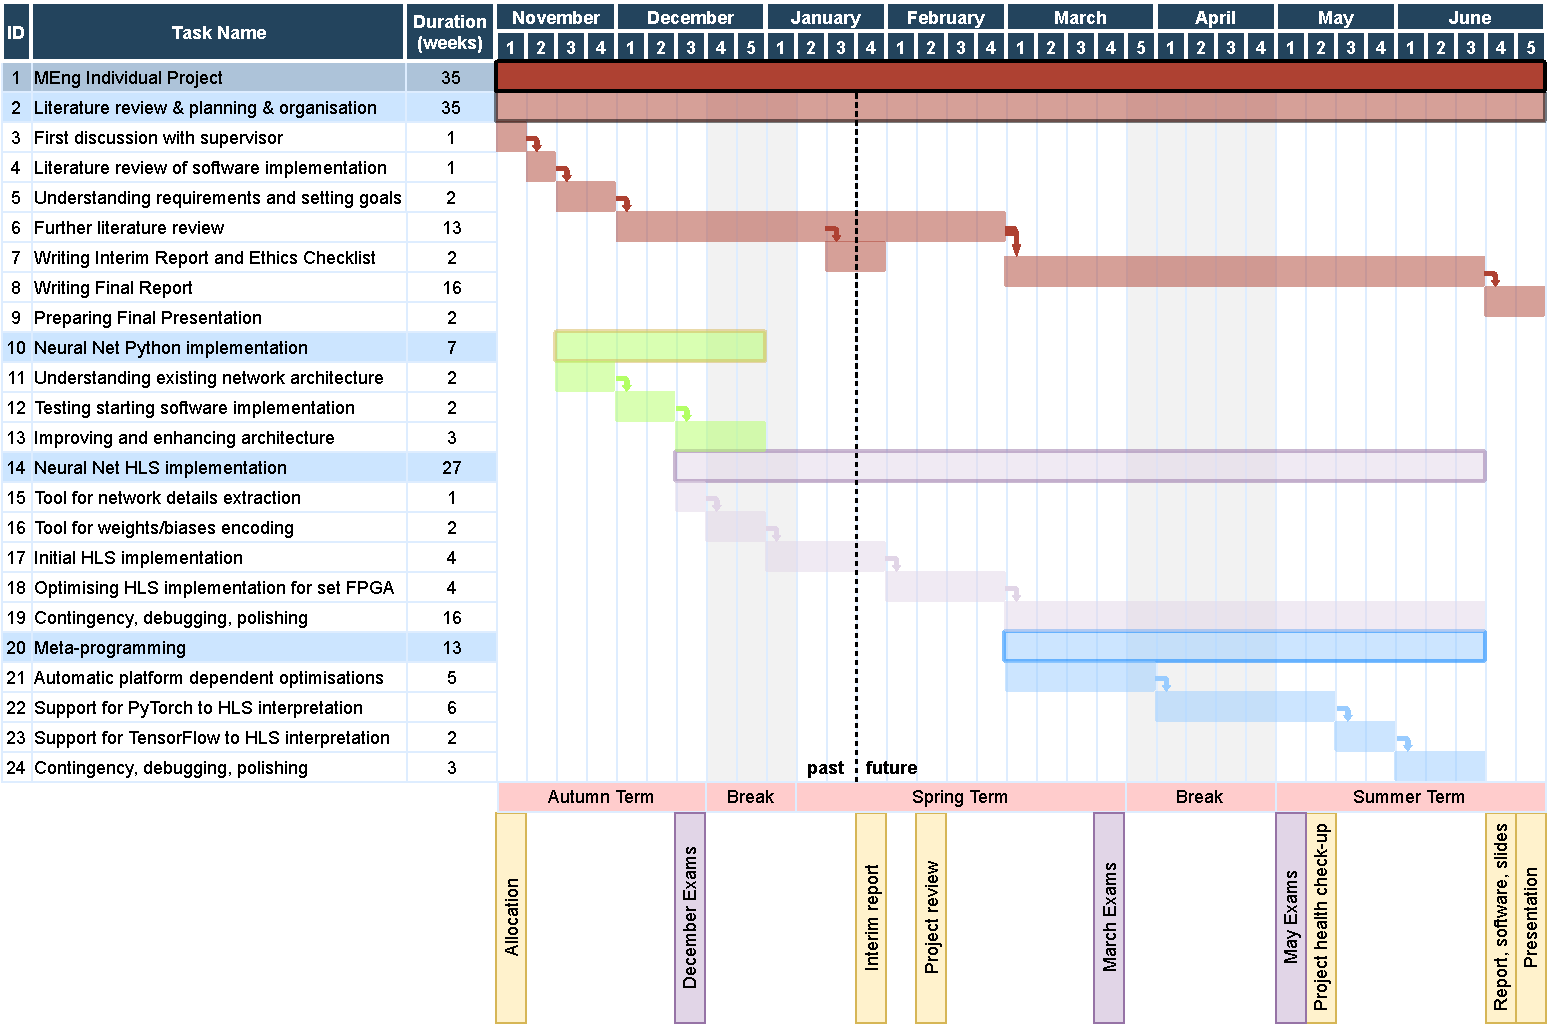
\includegraphics[trim={0cm 0cm 0cm 0cm}, width=1.2\textwidth, center]{project/gantt_chart.pdf}
  \caption{Project's Gantt chart representing initial plan of the work; past schedule has been updated to match ongoing progress accordingly}
  \label{fig:gantt-chart}
\end{figure}
\chapter{Implementation}
\chapter{Evaluation Plan}

This section outlines the proposed evaluation plan for the project. The first objective of developing and optimizing a state-of-the-art neural network in hardware can be evaluated quantitatively, while integrating it into the \textit{hls4ml} library and making it easy for new users to use requires a more qualitative approach.

\section{Quantitative results}
The following describes the quantities that are planned to be measured:

\begin{outline}
  \1 Classification accuracy for each designed neural network on a validation dataset
  \1 Inference latency and throughput when running on the target platform
  \1 Hardware resource utilization (exact values for comparison with other platforms and percentage of available resources for understanding limitations):
    \2 Block RAM (BRAM)
    \2 Ultra RAM (URAM)
    \2 Digital Signal Processing units (DSP)
    \2 Flip-Flops (FF)
    \2 Look-Up Tables (LUT)
\end{outline}

In the early stages of the project, the above quantities will be measured from the results from simulation and synthesis reports. At a later stage, the best designs will be run on actual hardware platforms to validate them under real-life use cases. The platform planned for this part is an Intel Stratix V FPGA hosted in a Maxeler MPC-X dataflow node with 8 Maia dataflow engines and 48 GB of DRAM.

Apart from clear design improvements, it is predicted that most evaluated designs will offer trade-offs between classification accuracy, inference throughput and hardware utilization. It is not possible to find a design that is superior in every way, hence a \textbf{Pareto front} will play a key role in understanding the overall performance and selecting configuration with specific needs in mind.

\section{Qualitative results}
Qualitative

\chapter{Ethical Considerations}\label{ethical}

The purpose of this project is to advance the next-generation particle physics experiments. There are two main aspects that need to be considered - the development of a hardware-mapped transformer neural network architecture and the easy-to-access translation and optimization toolchain for efficiently expressing networks in common machine learning frameworks.  

The first feature is aimed at a purely civilian, scientific audience and it is tailored towards particle collision datasets. With that in mind, it is important to mention that, as with most machine learning research, there is potential for a misuse of the acceleration techniques towards a military or malevolent application that could negatively impact the society (issues A in table \ref{tab:ethical-issues}). However, this also means that there is a low risk for new emerging threats; rather the already present ones could become more serious. Fortunately, this should result in existing harm prevention measures staying intact or solely requiring adjustments to their accuracy or speed thresholds.

With the second element's goal of making the creation and deployment of neural networks more accessible, it could be argued that this may in turn increase the number of physics experiments requiring high energy consumption, like those at LHC \cite{1-cernfacts}, thus negatively effecting the environment (issue B in table \ref{tab:ethical-issues}). However, this is considered a very low likely cause of action, as the research work of this project is aimed at helping already running experiments and more importantly, the negative environmental implications (for which there are various mitigation strategies \cite{Guida_2016, 2-capeans2017strategies}) are heavily outweighed by potential beneficial technological advancements coming from the scientific discoveries.

Despite the aforementioned ethical issues, the project is aimed at benefitting the open-source scientific community world-wide. Its outcome could lead to a much more accessible and efficient inference methods that are applicable in many domains outside particle physics.

\begin{table}[hpt]
  \centering
  \caption{Overview of potential categorized ethical issues with an indication of their applicability}
  \label{tab:ethical-issues}
  \begin{adjustbox}{center}
  \def\arraystretch{1.5}
  \begin{tabular}{|l||l|c|}
  \hline
  \rowcolor[HTML]{DAE8FC} 
                                                                                                           & Involvement of...                                                                       & \multicolumn{1}{l|}{\cellcolor[HTML]{DAE8FC}Exists?} \\ \hline\hline
  Humans                                                                                                   & human participants                                                                      & No                                                   \\ \hline
  \rowcolor[HTML]{ECF4FF} 
  \cellcolor[HTML]{ECF4FF}                                                                                 & personal data collection and/or processing                                              & No                                                   \\ \cline{2-3} 
  \cellcolor[HTML]{ECF4FF}                                                                                 & collection and/or processing of sensitive personal data                                 & No                                                   \\ \cline{2-3} 
  \rowcolor[HTML]{ECF4FF} 
  \cellcolor[HTML]{ECF4FF}                                                                                 & processing of genetic information                                                       & No                                                   \\ \cline{2-3} 
  \cellcolor[HTML]{ECF4FF}                                                                                 & tracking or observation of participants                                                 & No                                                   \\ \cline{2-3} 
  \rowcolor[HTML]{ECF4FF} 
  \multirow{-5}{*}{\cellcolor[HTML]{ECF4FF}Personal data}                                                  & further processing of previously collected personal data                                & No                                                   \\ \hline
  Animals                                                                                                  & animals                                                                                 & No                                                   \\ \hline
  \rowcolor[HTML]{ECF4FF} 
  \cellcolor[HTML]{ECF4FF}                                                                                 & developing countries                                                                    & No                                                   \\ \cline{2-3} 
  \cellcolor[HTML]{ECF4FF}                                                                                 & low and/or lower-middle income countries                                                & No                                                   \\ \cline{2-3} 
  \rowcolor[HTML]{ECF4FF} 
  \multirow{-3}{*}{\cellcolor[HTML]{ECF4FF}\begin{tabular}[c]{@{}l@{}}Developing\\ countries\end{tabular}} & putting the individuals taking part in the project at risk                              & No                                                   \\ \hline
                                                                                                           & elements that may cause harm to the environment, animals or plants                      & *                                                    \\ \cline{2-3} 
  \multirow{-2}{*}{Environment}                                                                            & \cellcolor[HTML]{ECF4FF}elements that may cause harm to humans                          & \cellcolor[HTML]{ECF4FF}*                            \\ \hline
  \cellcolor[HTML]{ECF4FF}                                                                                 & potential for military applications                                                     & No                                                   \\ \cline{2-3} 
  \rowcolor[HTML]{ECF4FF} 
  \cellcolor[HTML]{ECF4FF}                                                                                 & strictly civilian application focus                                                     & Yes                                                  \\ \cline{2-3} 
  \cellcolor[HTML]{ECF4FF}                                                                                 & goods or information requiring export licenses                                          & No                                                   \\ \cline{2-3} 
  \rowcolor[HTML]{ECF4FF} 
  \multirow{-4}{*}{\cellcolor[HTML]{ECF4FF}Dual use}                                                       & affection of current standards in military ethics                                       & No                                                   \\ \hline
                                                                                                           & potential for malevolent/criminal/terrorist abuse                                       & *                                                    \\ \cline{2-3} 
                                                                                                           & \cellcolor[HTML]{ECF4FF}information on/or the use of sensitive materials and explosives & \cellcolor[HTML]{ECF4FF}No                           \\ \cline{2-3} 
  \multirow{-3}{*}{Misuse}                                                                                 & technologies that could negatively impact human rights standards                        & *                                                    \\ \hline
  \rowcolor[HTML]{ECF4FF} 
  \cellcolor[HTML]{ECF4FF}                                                                                 & software for which there are copyright licensing implications                           & No                                                   \\ \cline{2-3} 
  \multirow{-2}{*}{\cellcolor[HTML]{ECF4FF}Legal}                                                          & information for which there are data protection or other legal implications             & No                                                   \\ \hline
  Other                                                                                                    & \cellcolor[HTML]{ECF4FF}anyother ethics issues that should be taken into consideration  & \cellcolor[HTML]{ECF4FF}No                           \\ \hline
  \end{tabular}
  \end{adjustbox}
\end{table}
% \chapter{Conclusion}\label{conclusion}
This work provides important insights into reconfigurable acceleration of transformer neural networks for ultra-low latency applications like high energy physics. The proposed solutions cover the whole development spectrum, from software architecture design, through various optimization techniques, to efficient hardware mapping of the neural network models. In this chapter, the main technical contributions are firstly summarized, followed by a discussion covering the existing limitations discovered during our research. Finally, several possible extensions that could improve upon our work are covered.

\section{Achievements}
This project contributes to the following research areas:

\begin{itemize}
  \item \textbf{Hardware-Aware Neural Network Design}: We explore two neural network architectures, which combine ideas from state-of-the-art solutions and transform them into components that can be efficiently mapped to FPGAs while offering cutting-edge accuracy. The analyzed aspects involve weight and bias fusing for normalization, splitting of fully-connected layers, and preventing numerical instability in softmax activation function. To allow for an easier reasoning about the architectures, analytical models covering latency and DSP slices were developed.

  \item \textbf{Efficient Hardware Mapping}: We propose novel hardware blocks for tensor multiplication using Einstein Notation as well as latency and resource optimized log softmax and SiLU activations. On top of that, we further expand \hlsml library with efficient and customizable self-attention and transformer layers. We also introduce improvements to the fully-connected layer and the unit responsible for storing results of arbitrary precomputed functions. The resulting hardware design achieves nanosecond latency with classification quality comparable to GPU and CPU implementations that are run around thousand times slower.

  \item \textbf{Quantization-Aware Training}: We analyze existing solutions for quantization-aware training and adapt the most suitable framework to transformer neural networks. The conducted experiments highlight the best performing fixed-point representations and highlight potential pitfalls in very complex neural networks.

  \item \textbf{Post-Training Quantization}: We develop a novel algorithm for post-training quantization that can be used with existing models and target any hardware platform. Thanks to its user-defined parameters, the search can be configured to prioritize accuracy over resource utilization or vice-versa. Evaluation on the proposed models results in a nearly \nicefrac{2}{3} reduction of total bit-widths with negligible accuracy decrease.
\end{itemize}

\section{Limitations}
Due to the scope of the project, there was no extensive hyperparameter search involved in any of the neural network architectures. Further tuning might allow for better results, which can have a cascading effect on the rest of this report's analysis because the researched areas are tightly coupled. In other words, more optimized software models lead to better performing hardware implementations, which can be further amplified by carefully quantizing them during or after training. On that topic, the developed post-training quantization algorithm assumes high correlation between subsequent neural network layers. Although this was proven to be the case in our analysis, it might not generalize to every network type.

The more complex of the discussed transformer architectures was not able to be synthesized as a pipelined design using HLS due to the inherent intricacy of generating pipelined models. The serial implementation offers an interesting trade-off of a design that runs slower but requires substantially less resources. However, many real-life applications operate under strict latency constraints, which could not be met due to the existing limitations of the HLS process and the fundamental issue of transformer's complexity.

\section{Future Work}
There are four main areas that our work could be expanded upon, which involve modifying the transformer layer, especially the self-attention mechanism, enhancing the post-training quantization method, adapting existing High-Level Synthesis optimization tools, and experimenting with other datasets.

\subsection{Alternative Transformer Design}
There is an ongoing research into alternative transformer architectures, which improve upon the quadratic complexity of self-attention, that has proven to be the main challenge of accelerating transformers. Some solutions involve low-rank approximations, sparsity, memorization, or various other techniques, summarized in figure \ref{fig:transformer-landscape} \cite{81-tay2020efficient}. To tackle the complexity problem, a recent work also goes as far as exploring completely removing the self-attention layer \cite{82-mikuni2021point}.

\begin{figure}[hpt!]
  \centering
  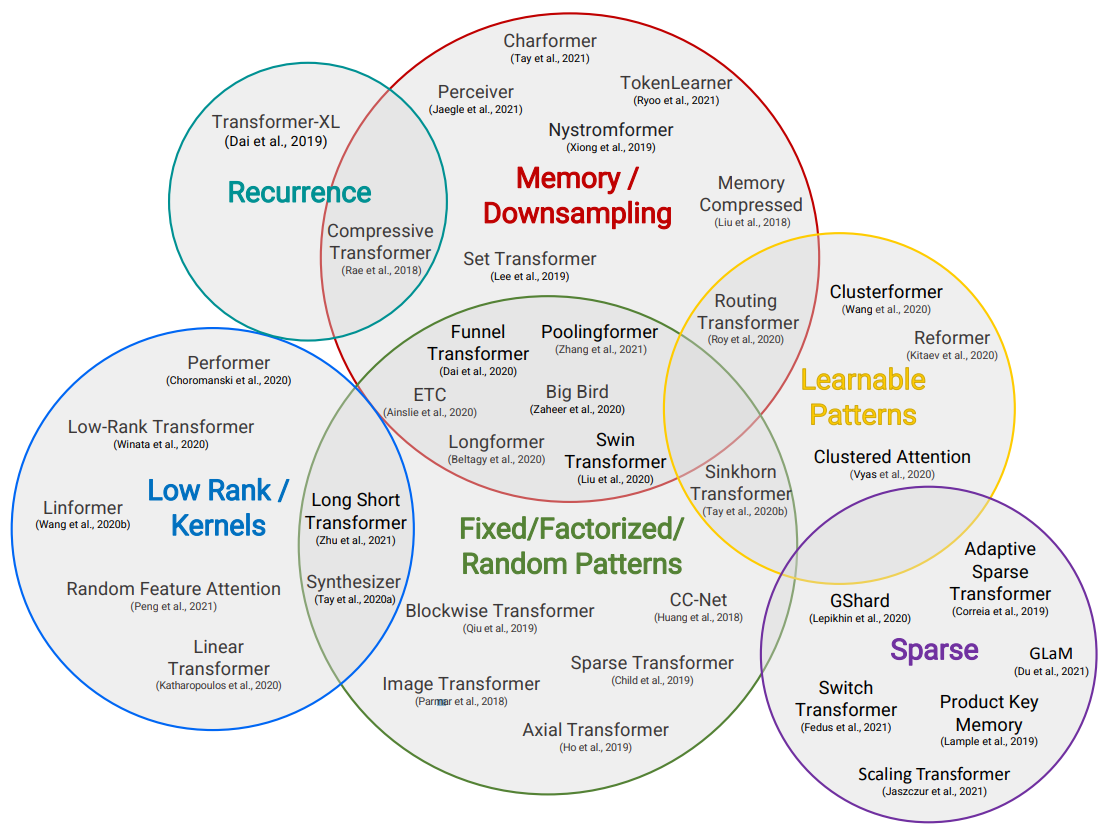
\includegraphics[trim={0cm 0cm 0cm 0cm}, clip, width=0.7\textwidth, center]{conclusion/transformer_landscape.png}
  \caption{Landscape of efficient transformer architectures.}
  \label{fig:transformer-landscape}
\end{figure}

Aside from changes to self-attention, trained transformer models could be compressed using techniques like pruning to decrease the number of stored weights which can improve the inference speed and reduce hardware utilization. Additionally, the already optimized batch normalization layers could be further improved by fusing with linear layers to reduce the overall complexity. Finally, recent automatic methods of finding efficient transformer configurations \cite{83-tsai2020finding,84-su2021vitas:} could help with the hardware-aware architecture search challenge.

\subsection{Post-Training Quantization Advancements}
The proposed post-training quantization algorithm could base its resource estimations on an analytical model to achieve more accurate predictions without compromising the search time. A new metric of energy-consumption could also be taken into consideration to accommodate mobile or embedded platforms' limitations. In order to accelerate the search process while potentially improving its findings, the approach could also benefit from a faster simulation and awareness of tested configurations' positions with regard to the underlying Pareto front or Roofline Model.

\subsection{Automatic High-Level-Synthesis Optimizations}
A recent High-Level Synthesis framework called ScaleHLS \cite{ye2021scalehls} promises to generate efficient RTL designs from HLS C++ or directly from PyTorch thanks to the use of optimizations at different levels of abstraction of the underlying Multi-Level Intermediate Representation (MLIR) \cite{mlir} used for PyTorch \cite{86-llvm2020torch-mlir}. This tool was explored during the project, but similarly to the discussed quantization-aware training methods, it does not support the self-attention layer in case of the direct PyTorch model optimization. As for trying it on the already developed HLS implementation, the size and the deep hierarchy involved in this work exceeds the complexity that ScaleHLS can handle. Nonetheless, further improvements might allow this framework to reduce the development time between designing a transformer architecture using \hlsml and testing its hardware implementation, supporting the objective of this work.

\subsection{Other Datasets}
Both of the datasets used in this project involve classification of five jet categories. However, other examples in the literature often discuss problems with fewer categories, for instance top-tagging, which is an approach to identifying top quarks. Simpler problems are likely to require less complex architectures - an area of the design space that this work proves to be optimal for transformers.

%//////////////////////////////////////////////////////
% at the end, CHECK:
% hyphens,
% 3rd person s in verbs,
% remaining todos,
% ugly page breaks,
% axis and titles in figures,
% correct some references to evaluation to be more specific (find all of them),
% change explanation in (brackets) to footnotes (always?),
% ensure no pre-training quantization but quantization-aware training,
% ensure network names like CNN, TNN are used consistently + no capital letters in convolutional nn, transformer nn,
% \begin{appendices}

\chapter{HLF dataset features distribution}
\begin{figure}[hpt!]
  \centering
  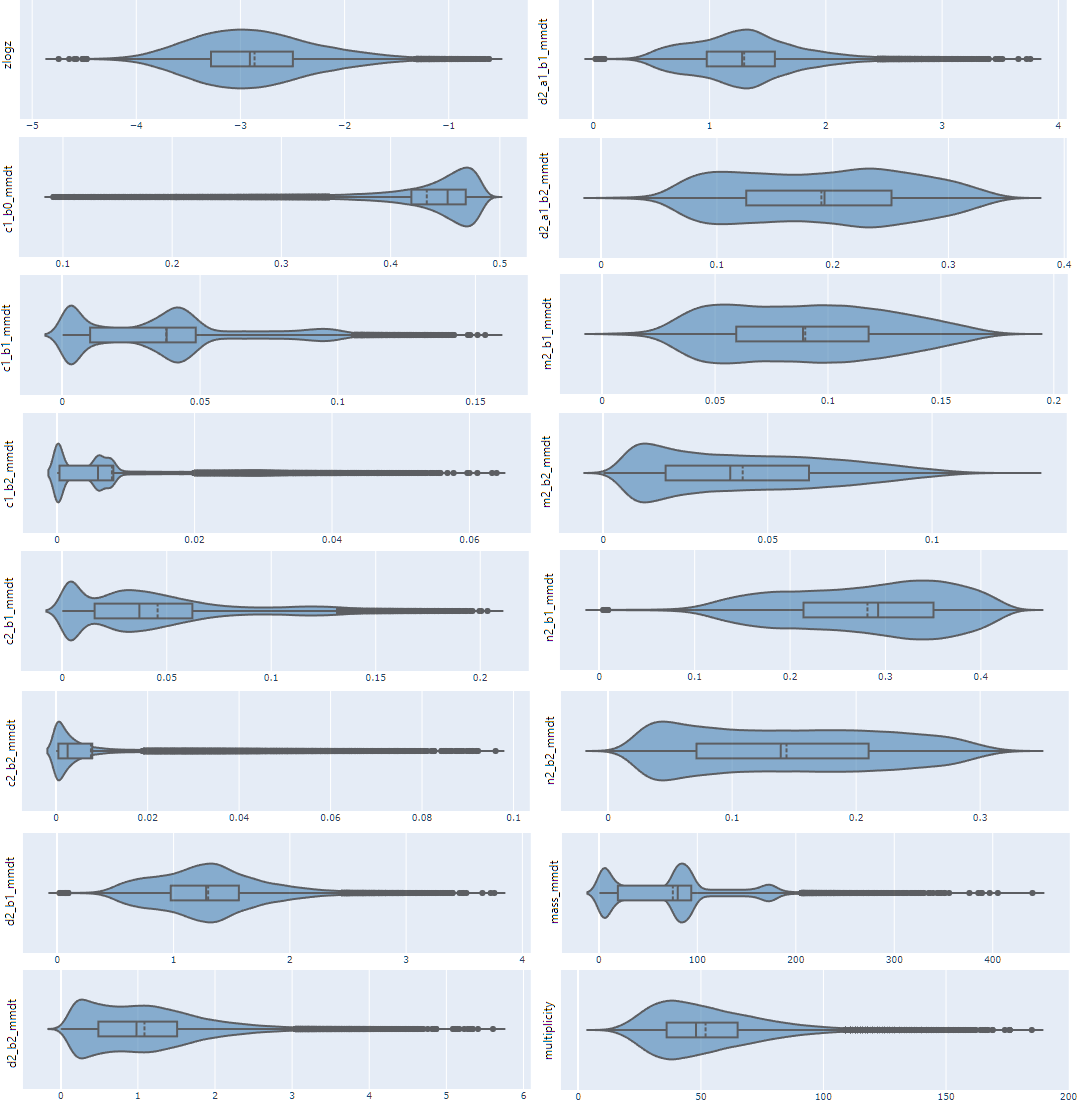
\includegraphics[trim={0cm 0cm 0cm 0cm}, width=1.0\textwidth, center]{background/distributions.png}
  \caption{Representation of the distributions of feature values in the HLF dataset.}
  \label{fig:distributions-hlf}
\end{figure}


\chapter{HLF dataset features distribution}
\begin{figure}[hpt!]
  \centering
  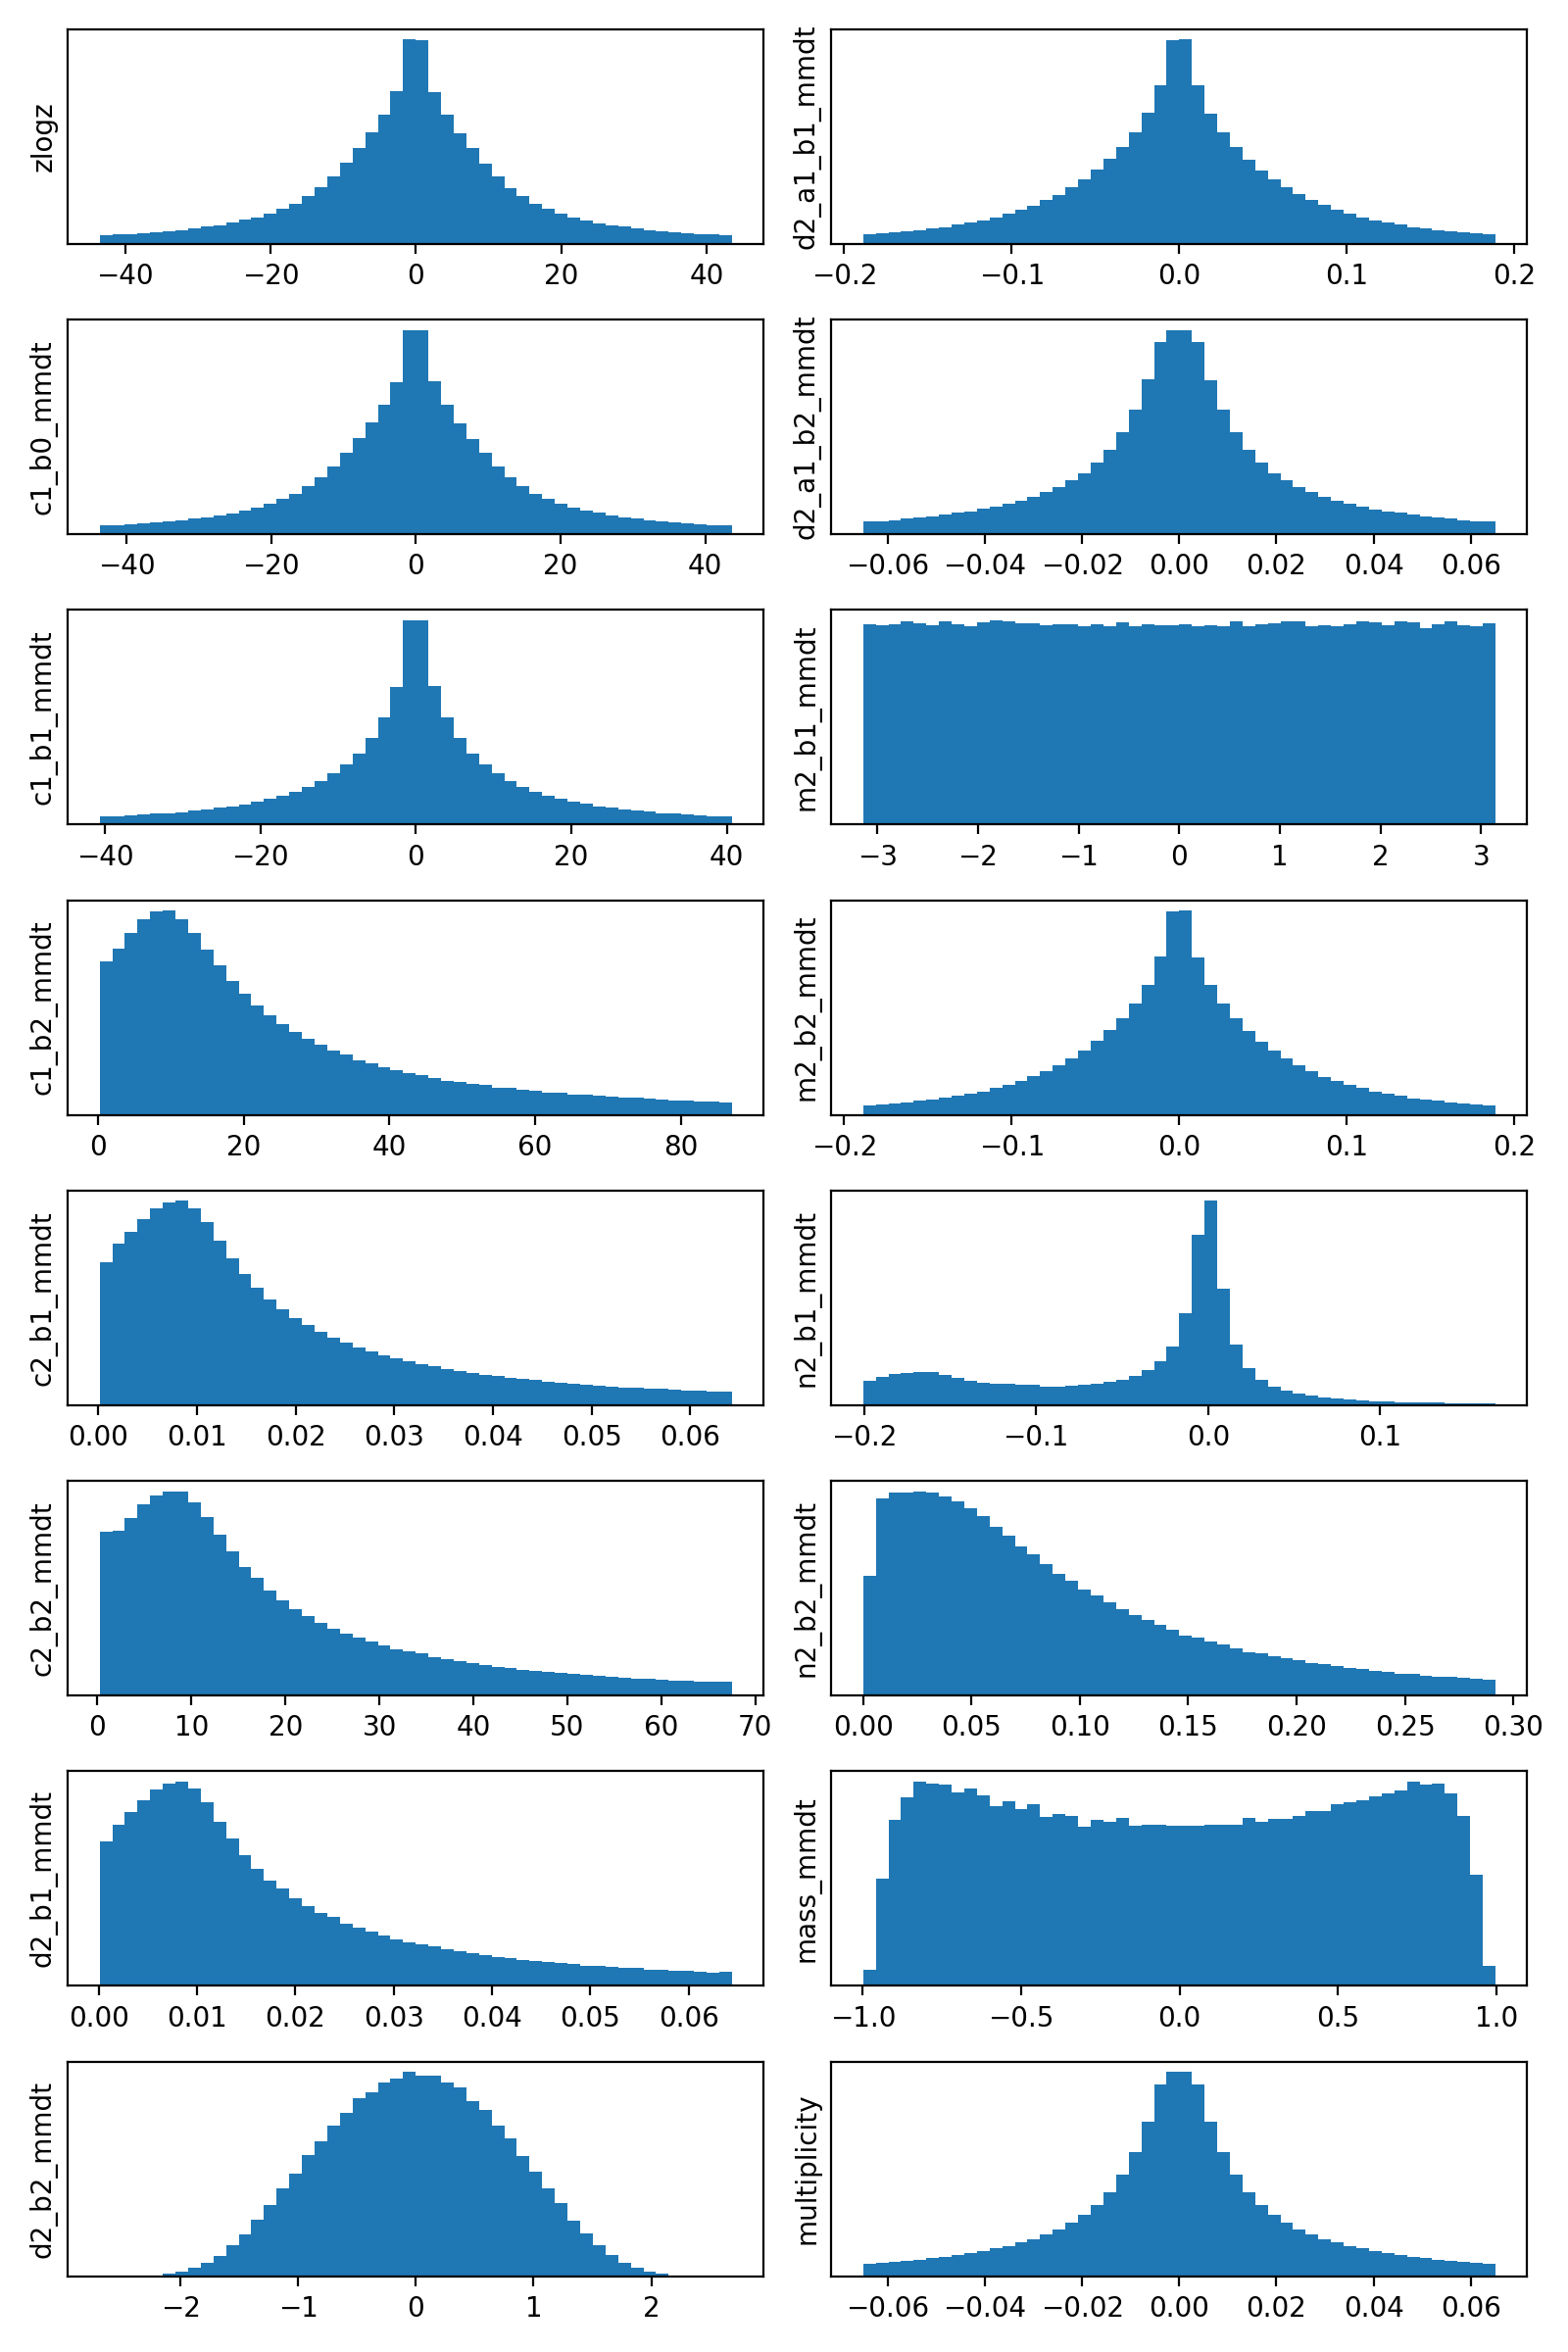
\includegraphics[trim={0cm 0cm 0cm 0cm}, width=0.7\textwidth, center]{../logs/constituent_distribution.png}
  \caption{Representation of the distributions of feature values in the constituent list dataset.}
  \label{fig:distributions-constituent}
\end{figure}

\end{appendices}

\bibliographystyle{unsrtnat}
\bibliography{references/references}

\listoftodos[Notes]

\end{document}